% Standalone supplementary material (own page and line numbers from 1).
% In Overleaf: Menu -> Main document -> supplementary.tex, then Recompile; switch back to main.tex for the paper.
% "Eq. (3) of the main paper"-style references come from main.aux via xr-hyper; latexmkrc compiles main.tex
% first when main.aux is missing or stale, so both work in Overleaf and with a local `latexmk -pdf supplementary.tex`.

\documentclass[10pt,twocolumn,letterpaper]{article}
\usepackage[review]{cvpr}
%% This file contains a number of tweaks that are typically applied to the main document.
%% They are not enabled by default, but can be enabled by uncommenting the relevant lines.

%%
%% Packages used by the STAGS draft (cvpr.sty already loads xcolor, graphicx, amsmath, amssymb, booktabs,
%% natbib, etoolbox, caption, subcaption, cleveref and enumitem).
%%
\usepackage{bm}
\usepackage{multirow}
\usepackage{siunitx}

%%
%% Draft marking: every addition after the (final) abstract is set in blue, including floats, captions,
%% tables and the bibliography. \normalcolor is redefined because LaTeX resets floats to it.
%%
\newcommand{\draftblue}{\color{blue}\renewcommand{\normalcolor}{\color{blue}}}


%%
%% Official support for 2-column teaser figure
%%
\usepackage{cuted} %< for strip environment

%%
%% For auto-referencing of figures (see fig/teaser.tex and \label{} therein) 
%%
\usepackage{currfile} %< for \currfilebase macro

%%
%% References across the paper/supplement boundary: the printed text says where the target is
%%
\newcommand{\suppref}[1]{supplementary~\cref{#1}}
\newcommand{\mainref}[1]{\cref{#1} of the main paper}

%%
%% caption and (global) spacing overrides
%%
\usepackage{caption} %< for "\captionof" commands (teaser)
% \setlength{\abovecaptionskip}{.5em} % space above caption
% \setlength{\belowcaptionskip}{1em} % space below caption

%%
%% Do not stretch vertical space to fill short columns (avoids a large gap
%% under the "Abstract" heading when the next section moves to the next column)
%%
\raggedbottom

%%
%% Inline annotations; for predefined colors, refer to "dvipsnames" in the xcolor package:
%% https://tinyurl.com/overleaf-colors
%%
\newcommand{\red}[1]{{\color{red}#1}}
\newcommand{\todo}[1]{{\color{red}#1}}
\newcommand{\TODO}[1]{\textbf{\color{red}[TODO: #1]}}
%%
%% Disable for camera ready / submission by uncommenting these lines:
%%
% \renewcommand{\TODO}[1]{}
% \renewcommand{\todo}[1]{#1}

%%
%% Work harder in optimizing text layout. Typically shrinks text by 1/6 of page, enable
%% it at the very end of the writing process, when you are just above the page limit.
%%
% \usepackage{microtype}

%%
%% Fine-tune paragraph spacing.
%%
% \renewcommand{\paragraph}[1]{\vspace{.5em}\noindent\textbf{#1.}}

%%
%% Globally adjusts space between figure and caption.
%%
% \setlength{\abovecaptionskip}{.5em}

%%
%% Allows "the use of \paper to refer to the project name"
%% with automatic management of space at the end of the word.
%%
% \usepackage{xspace}
% \newcommand{\paper}{ProjectName\xspace}

%%
%% Commonly used math definitions.
%%
% \DeclareMathOperator*{\argmin}{arg\,min}
% \DeclareMathOperator*{\argmax}{arg\,max}

%%
%% Tighten underline.
%%
% \usepackage{soul}
% \setuldepth{foobar}

%%
%% Reconfigure paragraph (tweaks spacing)
%%


\definecolor{cvprblue}{rgb}{0.21,0.49,0.74}
\usepackage{xr-hyper}
\usepackage[pagebackref,breaklinks,colorlinks,allcolors=cvprblue]{hyperref}
\externaldocument[]{main}

\def\confName{CVPR}
\def\confYear{2027}

\title{STAGS: Subtomogram Averaging with Gaussian Splatting}

\begin{document}
\clearpage
\setcounter{page}{1}
\maketitlesupplementary

% Own numbering (Sec. S1, Tab. S1, Fig. S1, Eq. (S1)), so supplement items cannot be mistaken for the paper's.
\setcounter{section}{0}
\setcounter{table}{0}
\setcounter{figure}{0}
\setcounter{equation}{0}
\renewcommand{\thesection}{S\arabic{section}}
\renewcommand{\thetable}{S\arabic{table}}
\renewcommand{\thefigure}{S\arabic{figure}}
\renewcommand{\theequation}{S\arabic{equation}}
\renewcommand{\theHsection}{S\arabic{section}}
\renewcommand{\theHtable}{S\arabic{table}}
\renewcommand{\theHfigure}{S\arabic{figure}}
\renewcommand{\theHequation}{S\arabic{equation}}

\section{Implementation details of STAGS}
\label{sec:suppl:method}

Values are those of the EMPIAR-10164 run; notation follows \mainref{sec:method}.
\Cref{tab:suppl:datasets} lists the only dataset-specific settings.

\begin{table}[t]
\centering
\footnotesize
\caption{\textbf{Dataset-specific settings} (EMPIAR-10164). $D$: particle diameter for the angular cap $d/D$; $V$: support volume that sets $K$ and the mask volume.}
\label{tab:suppl:datasets}
\setlength{\tabcolsep}{3pt}
\begin{tabular}{@{}ll@{}}
\toprule
point group $G$ & C6 \\
picks & surface normal, random spin \\
$p(R\mid\text{pick})$ & axis $90^\circ\pm10^\circ$ from normal \\
first search & global, after a 250-particle seed \\
$D$ / support radius & 250 / 250\,\AA \\
$V$ & 775,995\,\AA$^3$ (RELION mask) \\
pixel (bin 1) & 1.35\,\AA \\
mask $M$ & cylinder from axial profile \\
refinement band $d$ / cap $d/D$ & 3.5\,\AA\ / $0.80^\circ$ \\
\bottomrule
\end{tabular}
\end{table}
% src: stags/dataset.py DEFAULT
% EMPIAR-11830 column, removed from the submission for lack of final scores and a RELION baseline; to re-add, restore a
% second column (tabular lll, header "& EMPIAR-10164 & EMPIAR-11830 \\") with these values, all as actually run:
%   point group C1; picks template matching; prior uniform; first search local, +-12 deg; D / support radius 280 / 185 A;
%   V 11,828,213 A^3 (origin to be stated); pixel (bin 1) 1.91 A; mask thresholded own map;
%   refinement band 6.5 A / cap 1.33 deg; K 48,000; recipe E with exact translation, masked reference, separated motion.
% src (KW61627, x_kocalkm): runs/engine/chlamy11830/{dataset.json,ladder.json}; cycles_E/derived.json; cycles_E/cycles.log
%   (converged after cycle 4, 2026-11-16; defocus cross-half r only +0.46 -> +0.20, report if re-added)
% code: runs/engine/runC/run_c.py:main; src: runs/engine/pose_abc_adopt_20261113/blind/launch.json

\subsection{Data, extraction and optics}
\label{sec:suppl:method:data}

Inputs are RELION's tilt-series alignment, CTFFIND defocus, per-tilt scales and tilt exclusion, the initial surface-normal picks, and the half-set labels of RELION's final selection (300\,kV, $C_s=2.7$\,mm, amplitude contrast $w_a=0.1$).
% src: runs/engine/inputs/provenance.json ("tilt_series_contents", "selection_source", "pose_source", "a2")
% src: runs/engine/inputs/tomograms.star (rlnVoltage, rlnSphericalAberration, rlnAmplitudeContrast, rlnTomoTiltSeriesPixelSize, rlnTomoHand)
Crops are extracted by \texttt{relion\_tomo\_subtomo} (216\,px at bin 2 up to 6.5\,\AA; 384\,px at bin 1 for 5.5\,\AA\ and, without CTF multiplication, for the optics scan; 192\,px at bin 1 for map fits and refinement), using only $|\bm{\kappa}|\le1/d$.
% code: stags/engine.py:extract, HalfData.set_grid; scripts/lean_chain.py:main (initial extraction bin 2, box 256, crop 216), ladder_config (reextract bin 1, box 512, crop 384); runs/engine/runC/run_c.py:prep_half (crop 192; no_ctf crop RAW_CROP = 384), cycle_E (re-extraction crop 192)

The optics follow \mainref{eq:slice}, where $A_{ij}=\Gamma_{ij}R_i$ and $\mathbf{u}_{ij}=\Pi\,\Gamma_{ij}\mathbf{t}_i+\bm{\delta}_{ij}$, with $\Pi=[I_2\;\mathbf{0}]$, $\Gamma_{ij}$ the tilt rotation relative to the particle's first image and $\bm{\delta}_{ij}$ the motion shifts. The CTF is
\begin{equation}
\begin{aligned}
c_{ij}(\bm{\kappa})&=-\beta_j\big[\sqrt{1-w_a^2}\sin\chi_{ij}+w_a\cos\chi_{ij}\big],\\
\chi_{ij}&=\pi\lambda\,\Delta f_{ij}(\varphi)|\bm{\kappa}|^2-\tfrac{\pi}{2}C_s\lambda^3|\bm{\kappa}|^4,
\end{aligned}
\label{eq:ctf}
\end{equation}
% code: stags/relion5_io.py:_ctf_parts, wavelength; stags/relion5_io.py (Rt = Rz(ZRot) Ry(YTilt) Rx(XTilt)); stags/relion5_stags.py:relion_pose_decomposition
with per-tilt scale $\beta_j$ and defocus $\Delta f_{ij}(\varphi)$ combining mean defocus, astigmatism and the particle's depth.
The exposure filter is $e_j(\bm{\kappa})=\exp(-N_j/2N_e)$ with $N_e=0.245|\bm{\kappa}|^{-1.665}+2.81$~\cite{grant2015dose} at the midpoint exposure $N_j$ of tilt $j$.
% code: stags/relion5_io.py:_ctf_parts, wavelength (depth offset, dose = pre + 0.5 dose_per_tilt); stags/optics.py

The likelihood is evaluated on CTF-premultiplied crops: extracted crops are $\tilde{y}_{ij}=c_{ij}e_jy_{ij}$.
With $T_{ij}=(c_{ij}e_j)^2$, \mainref{eq:like} equals, up to a model-independent term,
\begin{equation}
\mathcal{L}=\sum_{i,j,\bm{\kappa}\neq0}\eta\,w\Big[T_{ij}|P_{ij}|^2-2\operatorname{Re}\big(\overline{P_{ij}}\,\tilde{y}_{ij}\big)\Big],
\label{eq:likepm}
\end{equation}
% code: stags/likelihood.py:image_objective (premultiplied: T|P|^2 - 2 Re(conj(P) D))
with Hermitian multiplicity $\eta$, so no division by the CTF is needed.
The weight $w$ is $\sum T/\sum|\tilde{y}|^2$ per one-pixel shell of the half's images.
% code: stags/likelihood.py:shell_noise_inverse; stags/train.py:fit_half (herm, shell 0 zeroed); stags/engine_search.py:noise_weights

\subsection{Initialization, densification and masks}
\label{sec:suppl:method:init}

To seed the mixture, each half back-projects 250 particles at their pick poses (C6 Wiener) and low-passes the map to 40\,\AA; isotropic Gaussians of width $d/3$ are sampled in proportion to squared positive density inside 250\,\AA, and one global amplitude is fitted in closed form.
% code: stags_engine.py:main (backproject band_A 16; lowpass 40); stags/engine.py:lowpass, initial_model, fit_amplitude; stags/train.py:seeds_from_volume; stags/relion5_io.py:reconstruct
The seed runs the 16\,\AA\ level on these particles until the map's non-cylindrical (lattice) fraction exceeds 0.12 and is stable (round 9 on both halves); the ladder then restarts from the pick poses.
% code: scripts/lean_chain.py:seed_config (rounds 30, lattice_stable delta 0.01, rounds 3), runs/engine/runC/run_c.py:run_ladder (--seed_lattice 0.12); stags/engine.py:noncylindrical_fraction; src: runs/engine/pose_abc_adopt_20261113/blind/lean/seed/h{1,2}/summary.json

Densification sets the target at level $d$ to $K(d)=\operatorname{round}(0.7\,V/(d/2)^3)$ (cap 50,000, never binding), from 1,061 at 16\,\AA\ to 26,119 at 5.5\,\AA.
% code: stags/engine.py:k_target_total; scripts/lean_chain.py (MASK_VOLUME_A3, K_CAP = 50000)
% src: scripts/lean_chain.py:45 (MASK_VOLUME_A3 = 775994.93); runs/engine/pose_abc_adopt_20261113/blind/lean/ladder/h{1,2}/summary.json (levels[].K_total)
At each level change, Gaussians lighter than 1\% of the median mass or outside the support are pruned; the widest Gaussians with $s_{\max}>d/3$ are then split, widest first, into two children at $\bm{\mu}\pm0.6\,s_{\max}\mathbf{v}$ along the long axis $\mathbf{v}$, with that width scaled by 0.8 and half the mass, until the target is reached; finally the heaviest $K(d)$ are kept.
% code: stags/engine.py:densify; scripts/lean_chain.py:ladder_config (no_densify_levels ["16"]); src: runs/engine/pose_abc_adopt_20261113/blind/lean/ladder/h{1,2}/summary.json (densify.residual_added = 0)
The fixed-pose fit starts with $K=48{,}000$, seeded likewise from the masked back-projection at the 5.5\,\AA\ poses.
% code: runs/engine/night_20261110/night.py:fit_cmd (--K 48000 --init voxel); stags/relion5_stags.py (init == "voxel": seeds_from_volume(VA * mask, lowpass_A 16); fit_scale kmax 1/20; init_model: no amplitude refit)

The particle mask $M$ is a cylinder about the symmetry axis whose height comes from the axial profile of the half's own back-projection at the 5.5\,\AA\ poses and whose radius makes it contain $V$, with a 6\,\AA\ cosine edge.
% EMPIAR-11830 (removed, re-add with the table column): For EMPIAR-11830, $M$ is instead the half's Gaussian map at the end of the ladder, low-passed to 8\,\AA\ and thresholded to the support volume $V$ (\cref{tab:suppl:datasets}), keeping the largest connected component, with a 6\,\AA\ cosine edge.
% code: scripts/dataset_final.py:model_mask
$V_{\mathrm{out}}=V_A(1-M)$ is recomputed at the current poses by every later stage.
% code: runs/engine/runC/run_c.py:prep_half (backproject wiener 0.05, sym C6, kmax 1/12); runs/engine/night_20261110/night.py:cylinder_mask_from_volume; stags/engine.py:HalfData.use_mask("sphere", 250); src: runs/engine/pose_abc_adopt_20261113/blind/kb/h1/prep.json (radius_A, fraction_of_box)

\Cref{tab:suppl:ladder} lists the levels of the resolution ladder.
The 16\,\AA\ search is global on a $10^\circ$ grid with exact projections, refined at $\pm5^\circ$ around the best 32; later levels score trilinear slices of a table of \mainref{eq:ft} around the previous top 32 and set the pose to the top candidate.
At 16 and 12\,\AA\ the halves share their transforms at $|\mathbf{q}|\le1/40$\,\AA$^{-1}$.
Map fits use Adam~\cite{kingma2015adam} (batches of 6 particles) over the top-$k$ candidates with renormalized posterior weights.
% code: stags/engine_search.py:so3_grid, posterior_cached, CachedEStep, posterior_sliced, local_offsets, sphere_grid, shift_nll; stags/slice_render.py:FourierVolume
% code: stags_engine.py:main (R0, t0 = Rk[:,0], tk[:,0]); stags/engine.py:join_partner; stags/engine_search.py (F[|k| <= 1/40] = 0.5 (own + other)); stags/slice_render.py:blend_low
% code: stags/engine.py:fit_soft, PlateauRule, _sample_rows; scripts/lean_chain.py:LADDER (max passes, tilt fraction 0.5)

\begin{table}[t]
\centering
\footnotesize
\caption{\textbf{Resolution ladder.} Rotation step, E-steps, candidates per map fit and shift radius/step.}
\label{tab:suppl:ladder}
% src: scripts/lean_chain.py:LADDER (rows for 16-5.5 A; the 4 A row is removed by --ladder_stop 5.5)
\setlength{\tabcolsep}{3pt}
\begin{tabular}{@{}rclcccc@{}}
\toprule
$d$ (\AA) & bin & search & step & E & top-$k$ & shift (\AA) \\
\midrule
16  & 4 & global & $5^\circ$ & 1 & 8 & 40 / 4 \\
12  & 4 & slices & $2.75^\circ$ & 2 & 8 & 40 / 3 \\
10  & 2 & slices & $2.29^\circ$ & 2 & 8 & 15 / 2.5 \\
8   & 2 & slices & $1.83^\circ$ & 3 & 4 & 10 / 2 \\
6.5 & 2 & slices & $1.49^\circ$ & 3 & 4 & 8 / 1.625 \\
5.5 & 1 & local $3^\circ$ & $0.5^\circ$ & 3 & 4 & 5 / 1 \\
\bottomrule
\end{tabular}
\end{table}

\subsection{Fixed-pose map fits}
\label{sec:suppl:method:fit}

With poses and corrections fixed, the data term of \cref{eq:likepm} is accumulated once on a twofold-oversampled 3D Fourier grid: each sample at $\mathbf{q}=A_{ij}^{\top}[\bm{\kappa};0]$ is spread onto nodes $\mathbf{q}_n$ with Kaiser--Bessel weights $b_n(\mathbf{q})$ (width 4, partition of unity),
\begin{equation}
\begin{aligned}
B_n&=\textstyle\sum\tfrac12\eta w\,b_n(\mathbf{q})\,\tilde{y}_{ij}\,e^{2\pi i\bm{\kappa}\cdot\mathbf{u}_{ij}},\quad
W_n=\textstyle\sum\tfrac12\eta w\,b_n(\mathbf{q})\,T_{ij},\\
\mathcal{L}_{\mathrm{KB}}&=\textstyle\sum_n W_n|F(\mathbf{q}_n)|^2-2\operatorname{Re}\big(\overline{F(\mathbf{q}_n)}B_n\big).
\end{aligned}
\label{eq:kb}
\end{equation}
% code: stags/normal_kb.py:build_kb_statistics, KBStatistics.objective, KBGrid.stencil
No deapodization is needed because $F$ is evaluated analytically at the nodes.
Each Adam step evaluates \mainref{eq:ft} at 262,144 randomly sampled occupied nodes, an unbiased estimate of $\mathcal{L}_{\mathrm{KB}}$, while the band widens linearly from $1/A_0$ to 1/2.7\,\AA$^{-1}$ over 60\% of the steps.
The cold fit uses $A_0=20$\,\AA\ (32 passes); refits during refinement use $A_0=6$\,\AA.
Outside density enters as $B_n\leftarrow B_n-W_nF_{\mathrm{out}}(\mathbf{q}_n)$.
% code: stags/normal_kb.py:KBGrid, build_kb_statistics, KBStatistics.objective; stags/train.py:fit_half (kcut; lr schedule; sample_size 262144; subtract mode 3; log_s clamp); runs/engine/night_20261110/night.py:fit_cmd (--lr_final 0.05); runs/engine/runC/run_c.py (ITERS, cycle_E: 6048, band_start 6.0); stags/gaussians.py:voxelize

\subsection{Local pose refinement}
\label{sec:suppl:method:p2}

At $k_{\mathrm{cut}}=1/3.5$\,\AA$^{-1}$, each particle tests 925 rotations ($0.5^\circ$ lattice in a $3^\circ$ ball) and shifts on a 1\,\AA\ lattice within 5\,\AA, scored with \mainref{eq:posterior} against the map multiplied by $M$, with $V_{\mathrm{out}}$ subtracted from the data.
The pose moves to the posterior mean of the top 8, with the rotation change capped at $d/D=3.5/250$\,rad ($0.80^\circ$) and the translation change at 3.5\,\AA; $\mathbf{t}_i$ is then refined by Gauss--Newton with the exact phase $e^{-2\pi i\bm{\kappa}\cdot\Pi\Gamma_{ij}\mathbf{t}}$.
Cycles stop when the median rotation change falls below half the cap ($0.40^\circ$) on both halves.
% src: runs/engine/runC/run_c.py:6 (stop rule: median P2 rotation move below half the 0.80 deg cap, 0.40 deg, on both halves)
% code: runs/engine/lean_20261110c/kb/p2_search.py (defaults step 0.5, theta 3, radius 5, sstep 1, update top8; --d 3.5 --exact_translation --mask_reference; cap_deg; refine_final_translation); stags/translation_refine.py:refine_translations; stags/engine.py:HalfData.subtract_outside, D_PARTICLE

\subsection{Optics scan}
\label{sec:suppl:method:optics}

For every tilt image $g$, the scan fits a defocus change $\delta f_g$, an astigmatism change $\bm{\alpha}_g$ and a scale $s_g$ to the crops without CTF multiplication by minimizing the whitened residual $\min_{s\ge0}\sum|\hat{y}_{ig}-s\,c_{ig}(\delta f,\bm{\alpha})\,e_gP_{ig}|^2$ at $|\bm{\kappa}|\le1/3$\,\AA$^{-1}$.
% code: runs/engine/night_20261110/swap/tilt_optics_scan.py (ctf_of, residual, best_scale; raw branch H = c2 e P; --no_outside)
$\delta f$ is scanned over $\pm2{,}000$\,\AA\ in 50\,\AA\ steps, with Gaussian priors toward the tomogram's change (250\,\AA) and between consecutive exposures (200\,\AA), solved by dynamic programming; $\bm{\alpha}$ is scanned on a coarse-to-fine grid.
The crops are then re-extracted with the updated optics; the scan repeats while the median change is at least 50\,\AA.
% code: runs/engine/night_20261110/swap/tilt_optics_scan.py (grid, Viterbi, astig coarse/fine, astig prior, scale_clamp, tomograms.star); runs/engine/runC/run_c.py:SCAN_FLAGS_E, cycle_E (SCAN_STOP_A = 50); src: runs/engine/pose_abc_adopt_20261113/blind/run_abc.log (cycle 4: |astig| median 50 / 50 A)

\subsection{Geometry and motion refinement}
\label{sec:suppl:method:p1}

With poses fixed, \mainref{eq:like} is minimized over a rotation (clamped to $1^\circ$) and a 2D shift (5\,\AA) per tilt image, by Adam, and over particle motion.
% code: stags/relion5_stags.py:tilt_geometry_tensors; runs/engine/v6/cycles/p1_polish.py (lr geom_ang 2e-4, geom_shift 0.02; clamps)
Each particle has a static offset $\mathbf{u}_i$, which moves only the Gaussians inside $M$, and a trajectory $\mathbf{m}_{ij}=\sum_{j'\le j}\mathbf{v}_{ij'}$, which also moves its surroundings, with RELION's polishing prior~\cite{zivanov2019polishing}
\begin{equation}
\Omega=\sum_{i,j}\frac{|\mathbf{v}_{ij}|^2}{(\sigma_v\Delta N_{ij})^2}+\sum_i\frac{|\mathbf{u}_i|^2}{\sigma_u^2}+\sum_{(i,i')\in\mathcal{N}}\sum_{j}\frac{|\mathbf{v}_{ij}-\mathbf{v}_{i'j}|^2}{\sigma_{\mathrm{nb}}^2},
\label{eq:motion}
\end{equation}
% code: stags/motion.py:MotionState (w_vel, w_nb, w_u); runs/engine/v6/cycles/p1_polish.py (sigma_vel 0.2, sigma_nb 0.5, sigma_u 10)
$\sigma_v=0.2$\,\AA\ per e/\AA$^2$, $\sigma_{\mathrm{nb}}=0.5$\,\AA, $\sigma_u=10$\,\AA, and $\mathcal{N}$ the particle pairs within 200\,\AA.
It is solved by damped Gauss--Newton with conjugate gradients, for at most ten passes.
% code: stags/motion.py:Layout, MotionState, separated_shift_grad_hess; runs/engine/v6/cycles/p1_polish.py (--motion --gn_cap 1.0 --background_once --separate_particle_translation; damping); stags/relion5_stags.py:tilt_prior_tensors (radius 200 A); runs/engine/runC/run_c.py:cycle_E (--rel_tol 5e-3 --max_passes 10 --min_passes 2)
Cross-half correlations were $r\ge0.99$ for per-tilt shifts, 0.85--0.93 for rotations and 0.91 falling to 0.53 for defocus changes; a correction group was admitted only at $r>0.8$.
% src: runs/engine/pose_abc_adopt_20261113/blind/run_abc.log; engine_rules.json (group admission r > 0.8)
% code: runs/engine/v6/cycles/p1_polish.py (exports geometry.pt, shifts.npz, poses.pt, base_shifts, total_shifts); runs/engine/runC/run_c.py:cycle_E (POSEFIX_ABC branch); runs/engine/lean_20261110c/kb/p2_search.py (base_shifts with corrected R_stage)


\section{Evaluation details}
\label{sec:suppl:eval}

The atomic model 5L93 is registered rigidly once, at 40--20\,\AA\ against RELION's merged map, and the same transform is used for every map.
% src: docs/results-stags-next-evaluation.md (model validation: registration 40-20 A, shared by every method)
Crossings are the first downward crossing between adjacent valid shells, linearly interpolated in frequency; the band mean over 3.6--3.28\,\AA\ weights the eight native shells equally.
% src: runs/engine/pose_abc_adopt_20261113/blind/comparison.json (crossing_definition, band_definition)
%STAGS's own two half maps share structure at 3.3--3.5\,\AA\ that RELION's maps do not contain (shared Gaussian texture or shared pose bias, not yet separated), which is why their mutual FSC is not used as a resolution estimate.
% src: docs/final-campaign-nov13.md (swap diagnostic: own gold FSC 0.45 at 3.5 A vs cross-FSC 0.22/0.19)
%Run~E is an earlier STAGS run with the previous recipe (3.343/3.396\,\AA). The final run used the same picks, ladder, budgets and stopping rule as run~E; besides the three pose corrections, 14 source or configuration files differ from run~E, so the difference between the two runs (0.074/0.145\,\AA\ in crossing, 0.036/0.052 in band mean) is not a clean ablation.
% src: docs/final-campaign-nov13.md (Fresh-run launch verification: fourteen hashes differ); runs/engine/pose_abc_adopt_20261113/completion_review.json (gain_vs_E_crossing_A, gain_vs_E_band_mean)

Because both STAGS half-maps are parameterized by continuous Gaussian kernels under identical densification schedules, they share a high-frequency spectral envelope at 3.3–3.5 Å absent from discrete voxel back-projections; cross-FSC against the opposite RELION-5 half-map eliminates this shared-basis correlation.

\section{Additional comparison with RELION-5}
\label{sec:suppl:visual}

\Cref{fig:views} shows both maps rendered identically and \cref{fig:slices} central sections without masking.
\Cref{fig:locres_cumulative} shows the distribution of the local-resolution values of \mainref{fig:locres} over all window centers inside the mask.
73\,\% (RELION-5) and 83\,\% (STAGS) of them are finer than 3.5\,\AA.
% src: docs/paper/fig_abc_provenance.json (local_resolution.summary: fraction_finer_than_3_5A relion 0.7336, stags 0.8310)
Windows coarser than 4\,\AA\ make up 13\,\% for RELION and 8\,\% for STAGS, and most of them lie within 10\,\AA\ of the mask boundary, so they reflect the mask edge rather than the structure.
% src: docs/paper/fig_abc_provenance.json (local_resolution.summary: fraction_coarser_than_4A 0.133 / 0.075; coarse_within_10A_of_mask_edge 0.72 / 0.79 vs all windows 0.48)
The RELION-5 paper does not list the regions of its Fig.~6C; for \mainref{fig:closeups} we recovered them by a joint silhouette match of 5L93 atoms and RELION density to the published panels, with leads of 1.59, 0.71 and 0.46\,px over the next distinct region.
% src: docs/paper/fig_abc_fig6c_regions.json; docs/final-campaign-nov13.md (Visual comparison)

\begin{figure}[t]
\centering
% src: fig/abc_views.png by scripts/paper_figures_abc.py; display parameters: docs/paper/fig_abc_provenance.json (display, views)
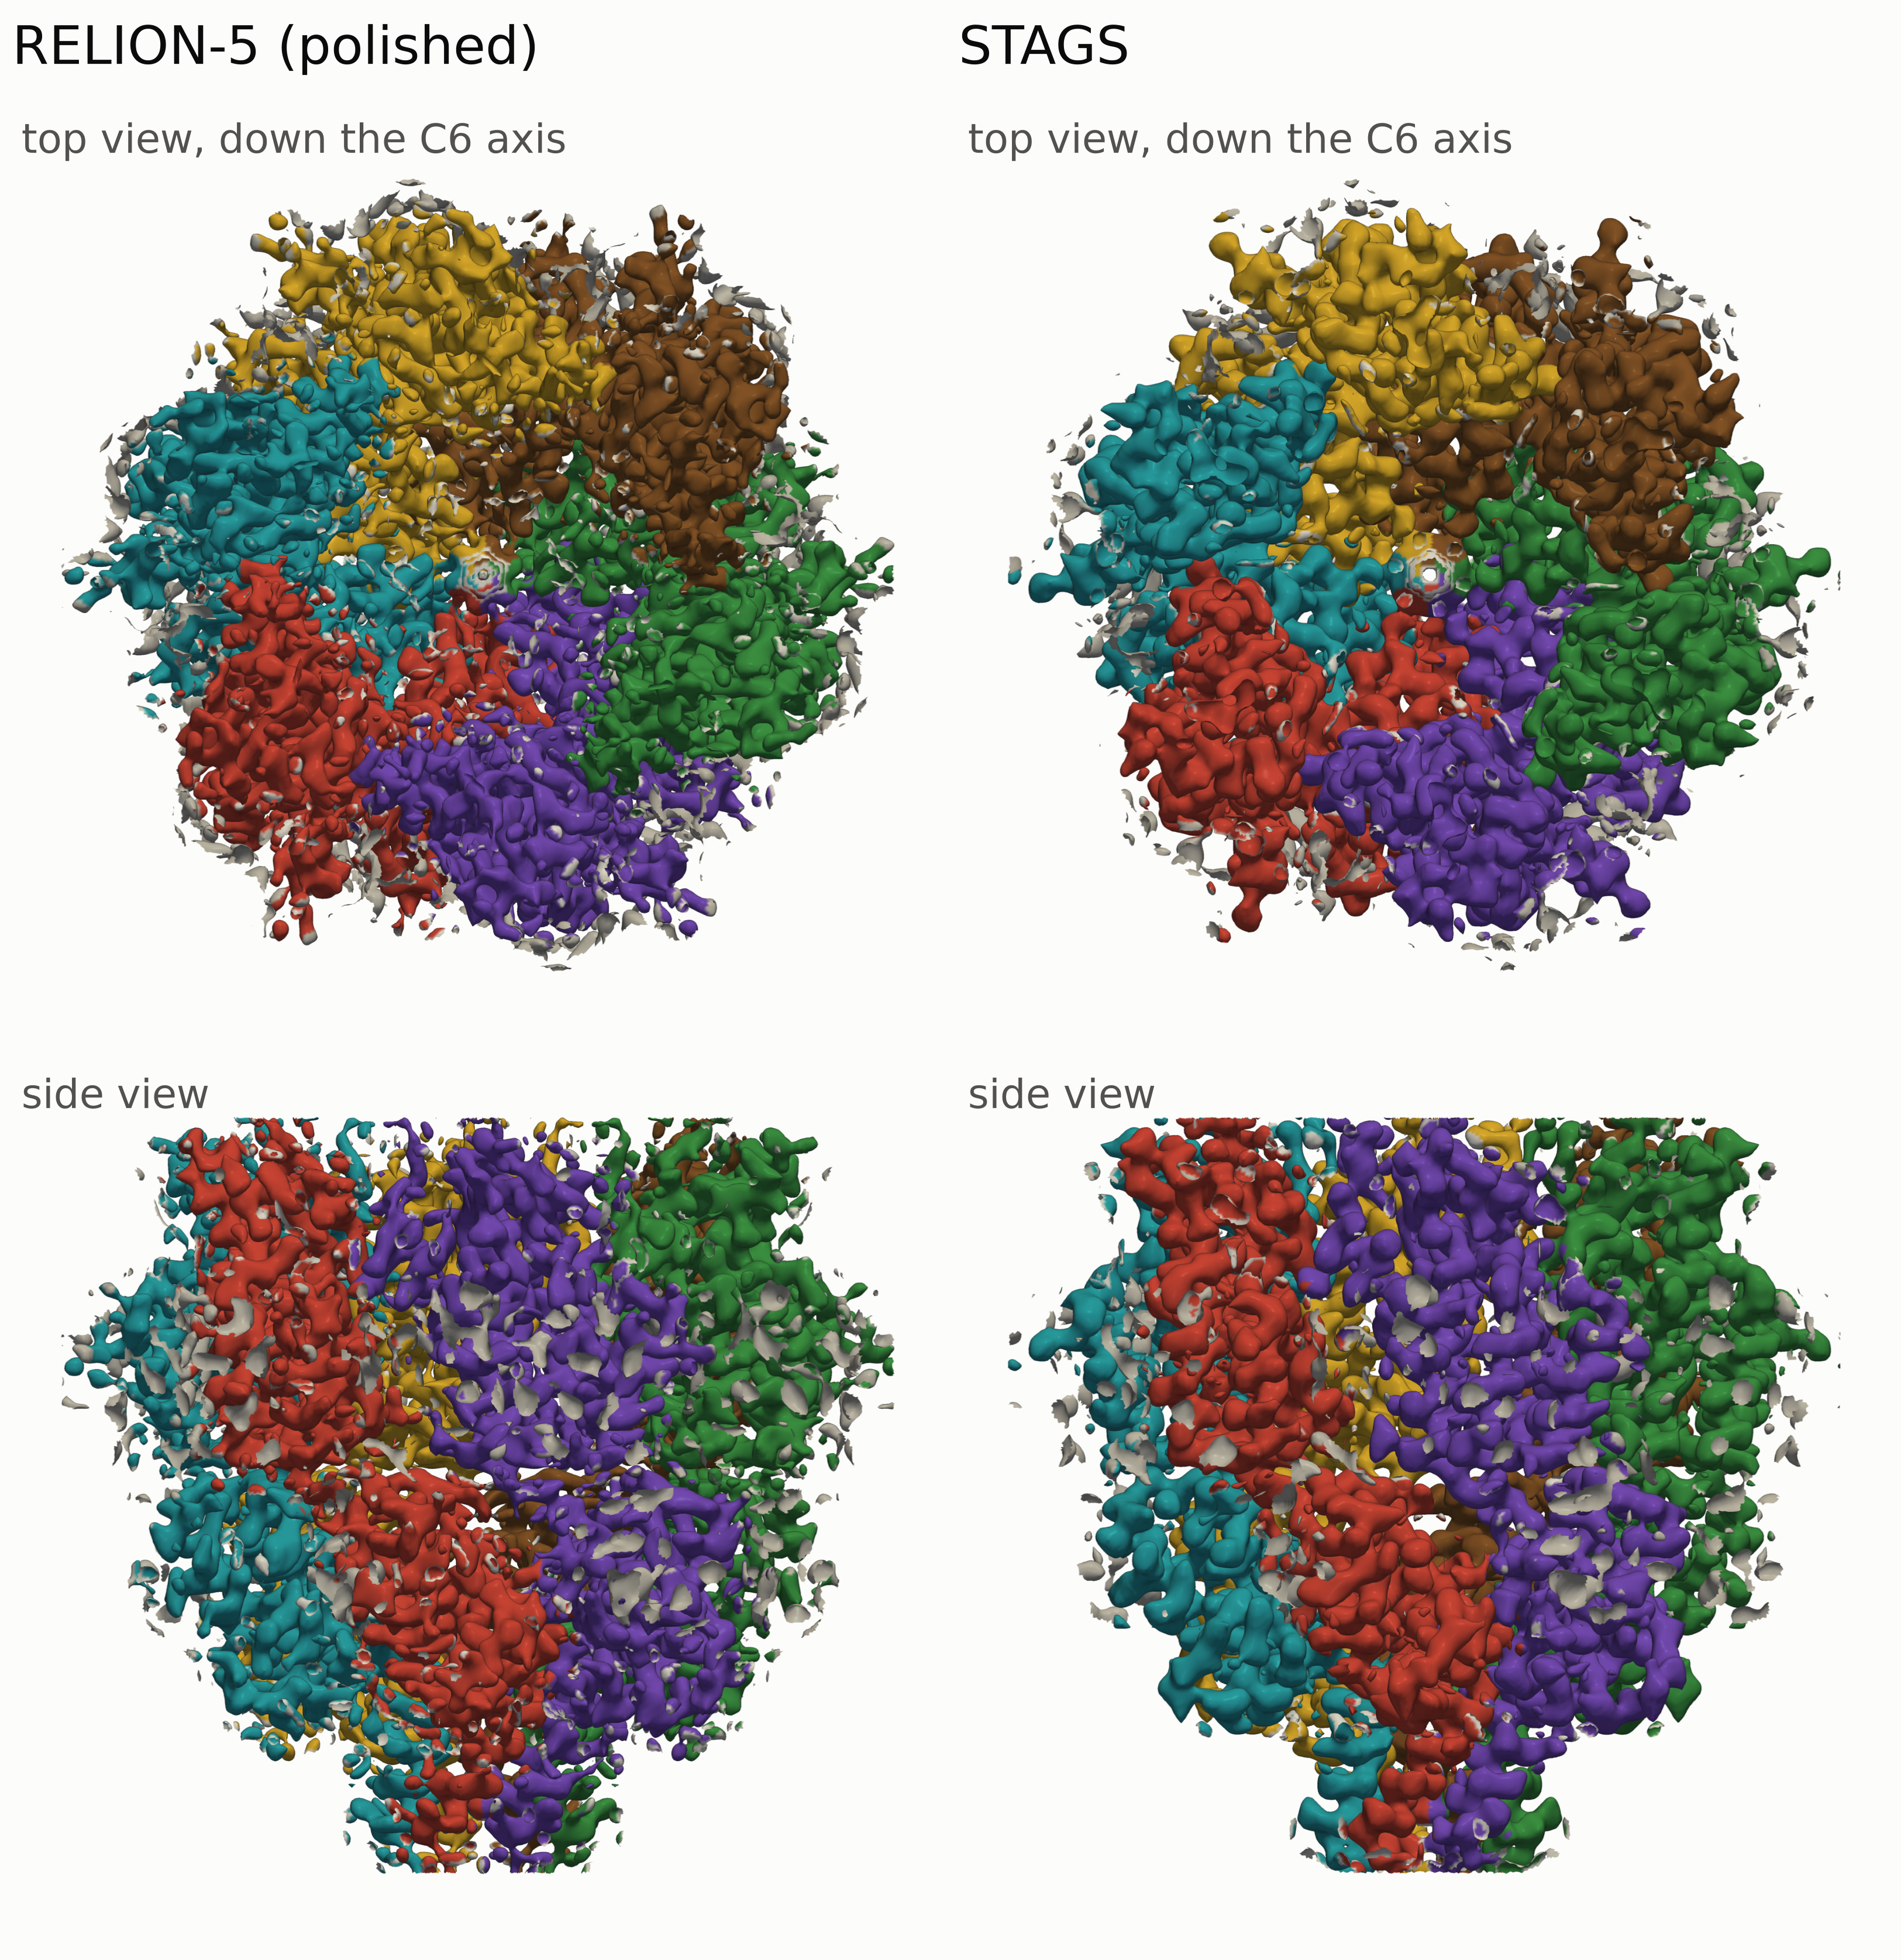
\includegraphics[width=\linewidth]{fig/abc_views.png}
\caption{\textbf{Identical renderings} of the central hexamer, RELION-5 (left) and STAGS (right), colored by nearest 5L93 subunit. Both: mean of normalized half maps, B-factor $-82.70$\,\AA$^2$, low-pass 3.5--3.1\,\AA, thresholded to the same 101,942\,\AA$^3$ in RELION's mask (the volume matching Fig.~6C of~\cite{burt2024relion5}).}
\label{fig:views}
\end{figure}

\begin{figure}[t]
\centering
% src: fig/abc_slices.png by scripts/paper_figures_abc.py (render --paper fig --only slices); docs/paper/fig_abc_provenance.json (slices: sections z,y,x = 106, 96, 95; gray range z = -2.18 ... 4.47); crop z,y,x = 66-147, 52-140, 52-140 px (mask_fsc > 0.5 box + 6 px)
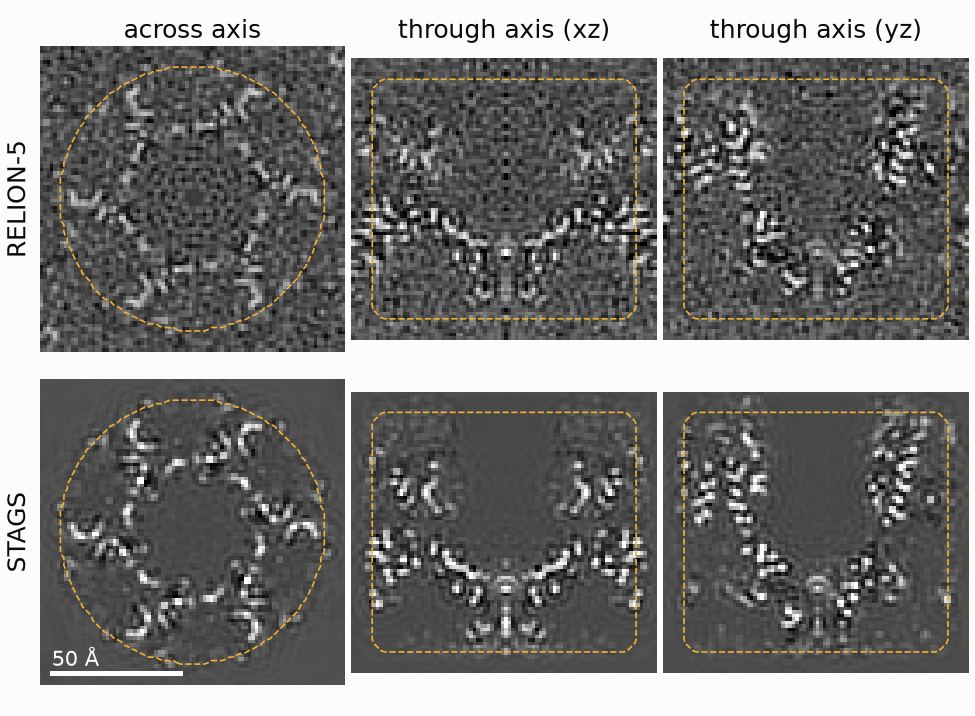
\includegraphics[width=\columnwidth]{fig/abc_slices.png}
\caption{\textbf{Central sections, unmasked,} cropped to RELION's mask (dashed). Filtering as in \cref{fig:views}; z-scored inside the mask; one gray scale (0.5--99.5\,\% of both maps).}
% src: docs/final-campaign-nov13.md (Visual comparison: "STAGS has no density outside its own mask")
\label{fig:slices}
\end{figure}

\begin{figure}[t]
\centering
% src: fig/abc_locres_cumulative.png by scripts/paper_figures_abc.py (render --paper); values: docs/paper/fig_abc_locres.csv (window centers with mask >= 0.5)
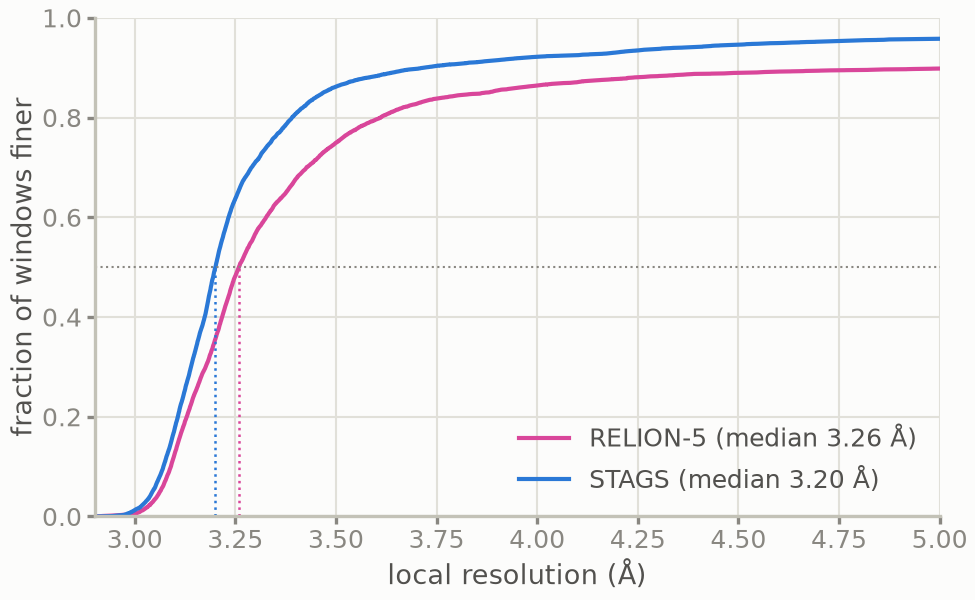
\includegraphics[width=\columnwidth]{fig/abc_locres_cumulative.png}
\caption{\textbf{Distribution of local resolution.}
For each map, the fraction of window centers inside RELION's mask whose local resolution is finer than a given value, from the same estimator as \cref{fig:locres}.
Each median is where its curve crosses one half.
The curves stay below 1 at 5\,\AA\ because some windows, mostly at the mask edge, are coarser.}
\label{fig:locres_cumulative}
\end{figure}


\section{Pose-correction ablation}
\label{sec:suppl:ablation}

\begin{table}[t]
\centering
\resizebox{\linewidth}{!}{%
\begin{tabular}{@{}lccccc@{}}
\toprule
& cross-FSC 0.143 (\AA) & gain vs.\ control (\AA) & mean FSC 3.6--3.28\,\AA & 5L93 & gate \\
Arm (one cycle from frozen run E) & half 1 / half 2 & half 1 / half 2 & half 1 / half 2 & FSC 0.5 (\AA) & decision \\
\midrule
% rows generated by scripts/paper_figures_cvpr.py (tab_ablation)
\csname @@input\endcsname fig/tab_ablation_rows.tex
\bottomrule
\end{tabular}}
\caption{\textbf{Pose-correction ablation:} one cycle continued from frozen run~E, scored as \mainref{tab:benchmark}. Gate: gain $>0.03$\,\AA\ on each half vs.\ control and frozen state, no worse 5L93 crossing. No arm passed; a+b+c ($^*$ failed on half~2) was adopted afterwards on band means.}
\label{tab:ablation}
\end{table}


\Cref{tab:ablation} tests three pose corrections, each in a matched one-cycle continuation from the frozen final state of run~E: (a)~exact Fourier-phase scoring of the final translation refinement, replacing bilinear interpolation, which drifts by 0.63\,\AA\ on known-answer fixtures where exact scoring drifts by 0.0002\,\AA; (b)~a masked Gaussian reference for the local pose search, with matching subtraction outside the mask; (c)~separate per-particle static translations and shared motion in polishing.
% src: docs/final-campaign-nov13.md (Step 1 recovery: 0.632614/0.625859 vs 0.000217/0.000210 A); runs/engine/posefix_20261113/recovery/report.json
The predeclared gate required a gain above 0.03\,\AA\ on each half, against both the continuation control and the frozen state, with no worse atomic agreement.
% src: engine_rules.json steps.posefix_20261113; docs/final-campaign-nov13.md (Frozen-E pose correction)
Alone, each change gains at most 0.021\,\AA; together they gain 0.082\,\AA\ on half~1 but only 0.015\,\AA\ on half~2, so the combination failed the gate.
% src: runs/engine/posefix_20261113/{a,b,c,abc}/result.json
Exact scoring inside the rotation-candidate ranking, evaluating every candidate, did not improve on the combination (0.064/0.013\,\AA) and was not adopted.
% src: runs/engine/pose_rank_exact_20261113/abc_exactrank/result.json; decision.json (blind_authorized=false)
We adopted the combination for the fresh run \emph{after} seeing these results: its mean FSC over 3.6--3.28\,\AA\ rose on both halves (+0.016/+0.017), its curves exceed the control's at every shell of that band, and its atomic agreement improved.
% src: docs/final-campaign-nov13.md (Explicit post-result adoption: +0.016170/+0.017196); runs/engine/pose_rank_exact_20261113/curve_diagnosis.json
The failed gate is not reclassified, and the selection after the result is part of why the benchmark is a development result rather than independent validation.

\section{Fixed-pose particle efficiency: details}
\label{sec:suppl:efficiency}

\paragraph{Withheld-tomogram study.}
The three splits withhold TS\_54, TS\_03 and TS\_45; the 250 training particles are drawn from the other four tomograms and 200 particles of the withheld tomogram are used only for image prediction.
% src: runs/native_limited250_20261103/selection.json (train TS_01/03/43/45; 250 train; 200 held out); docs/stags-limited-particle-study-matrix.md
The Gaussian map (48,000 Gaussians, 2,667 updates of 6 particles) is fitted to RELION's extracted particle images at 1.5$\times$ binning, with density outside the mask subtracted using a voxel map of the same 250 particles.
% src: engine_rules.json steps.A3_break_fixed_point.snr_gate.what; runs/step2_parity_20261103/score_primary/results.json (endpoint.recipe_differences)
It passes the predeclared margin of +0.01 FSC in every split, and its 5L93 crossing is slightly finer (7.08, 7.03, 7.05\,\AA\ against 7.23, 7.05, 7.16\,\AA).
% src: docs/results-limited250-three-study-20261103.md
The study's predeclared Gaussian arms (ray and wave models fitted to raw images at native sampling) failed against the voxel baseline (0.243 and 0.248 against 0.509); the reported recipe is an earlier one, substituted after that failure and scored under the same frozen gates.
% src: docs/results-limited250-primary-20261103.md
RELION-5 with 500 particles is better in all three splits (0.620, 0.601, 0.582), so the gain is not a halving of the particle count.
Image prediction on the withheld tomogram favors the Gaussian map (normalized squared error 0.99998 against 1.00074 in the first split), but an untrained Gaussian initialization already reaches most of that difference, and all methods explain almost none of the held-out signal.
% src: runs/native_limited250_20261103/native500_score/results.json (loss_over_observed_power); docs/results-limited250-primary-20261103.md (zero-update 0.99999)
All maps are scored against RELION's half-2 map, refined with the same poses, so the comparison is conditional on them.

\paragraph{Map-only control.}
The control fits the image-fit recipe's Gaussian initialization and schedule to the 250-particle voxel map.
% src: runs/native_limited250_20261103/control_v4_rules.json
It ran once, in the first split, without an adequacy gate, and scores 0.508 against 0.509 for the voxel map and 0.570 for the image-fitted Gaussians; its 5L93 crossing is much coarser (15.6\,\AA).
% src: runs/native_limited250_20261103/control_v4_outcome.json; map_only_control_v4/score/results.json
Three earlier versions failed the study's predeclared adequacy requirement, a relative $L_2$ error below 0.10 against the voxel map (1.15, 0.88 and 0.96); the 250-particle map is noise-dominated beyond 8\,\AA\ (97\,\% of its power), so a representation that does not copy its noise cannot meet that requirement.
% src: runs/native_limited250_20261103/map_only_control/decision.json (1.1506); controls_v2_outcome.json (0.883); control_v3_outcome.json (0.956; power beyond 8 A 0.973)
The control therefore supports, but does not prove, attributing the gain to the image-level fit.

\paragraph{Smoothing control.}
To test whether smoothing alone explains the gain, each 250-particle voxel map was filtered and scored with the same scorer: low-pass filters passing up to 8, 7, 6.5, 6 or 5.6\,\AA\ with a cosine edge to 1.15 times that frequency, and Gaussian blurs with B-factors of 50, 100, 200 and 400\,\AA$^2$.
The unfiltered scores are reproduced exactly (0.509, 0.479, 0.461).
In every subset the best filter is the blur with B = 100\,\AA$^2$, which raises the score by at most 0.006 (to 0.515, 0.483 and 0.465), against 0.570, 0.566 and 0.518 for the Gaussian map.
Stronger blurs and every low-pass filter lower it, down to 0.11--0.12 for the 8\,\AA\ low-pass, and the 5L93 crossing changes by at most 0.23\,\AA, coarser for the 8\,\AA\ low-pass and within 0.03\,\AA\ for the best filter.
Because the filter is chosen after scoring, this is an upper bound for isotropic smoothing of the voxel map.
% src: docs/paper/lowpass_control_summary.json; scripts/lowpass_control.py

\paragraph{Five-draw study.}
Five disjoint draws of 250 half-1 particles (nested in 500) with 200 further particles reserved compare raw-image Gaussian fits with a matched ridge-regularized voxel solver and with Gaussians fitted to each voxel-250 map.
% src: docs/results-stags-next-evaluation.md (particle-efficiency study)
Over 6.5--5.6\,\AA\ the Gaussian map exceeds the voxel-250 map by 0.175 (95\,\% CI [0.146, 0.203]) and the map-only fit by 0.137 [0.105, 0.169], and at 6.5\,\AA\ the voxel-500 map by 0.095 [0.064, 0.125].
% src: runs/particle_efficiency_20261102/results.json (comparisons A250, AG250, A500)
The map-only fits approximate their targets with a relative $L_2$ error of 0.98, so they are not an adequate smoothing control, and the Gaussian map predicts the reserved particles' images worse than the voxel-500 map in all five draws.
% src: runs/particle_efficiency_20261102/draw*/AG250/results.json (relative_map_l2 0.9789-0.9802); docs/results-stags-next-evaluation.md (reserved-particle prediction)

\section{Pipeline stage decisions}
\label{sec:suppl:part2}

Before the pose corrections of \cref{sec:suppl:ablation}, each stage of the pipeline was revisited with a predeclared keep rule on a short proxy: a cold map fit from the stage's output, or one refinement cycle, scored as in \mainref{sec:results:setup}.
\Cref{tab:part2} lists every tested change.
The proxies have a noise floor of about $\pm$0.02--0.03\,\AA, visible as gains of opposite sign on the two halves.
% src: docs/final-campaign-nov13.md (Part 2, stage2_fit note: proxy noise floor)
Two decisions were revised after their results and are marked as such: the coarse-to-fine schedule stops at 5.5\,\AA\ (saving 58\,min) although the rule rejected it on half~2 by 0.032\,\AA, after a later fresh run with that stop gave a better proxy (3.881/3.886\,\AA) and the spread between runs was seen to be about 0.1\,\AA; and the revised optics scan was kept although its one-cycle proxy was within noise, because the previous scan failed a known-answer test (median defocus offset 225\,\AA\ recovered for a true 400\,\AA, against 397\,\AA\ for the revised scan) and the revised scan roughly halves the defocus deviation from RELION's refined values (median 118/141\,\AA\ against 221/217\,\AA).
% src: docs/final-campaign-nov13.md (stage1_ladder caveat_recorded_after and decision_revised_after; stage4_scan known_answer_h1, relion_diagnostic, DEVIATION recorded after the result)

\begin{table}[h]
\centering
\resizebox{\linewidth}{!}{%
\begin{tabular}{@{}llccl@{}}
\toprule
Stage & Change & Proxy (\AA) & Reference (\AA) & Decision \\
& & half 1 / half 2 & half 1 / half 2 & \\
\midrule
% src: docs/final-campaign-nov13.md (Part 2: stage1_ladder)
Schedule & stop at 5.5\,\AA\ ($-58$\,min) & 3.907 / 4.041 & 3.924 / 4.009 & reject; kept after result \\
% src: docs/final-campaign-nov13.md (Part 2: stage2_fit)
Map fit & fit band ends at 3.0\,\AA & 3.948 / 3.993 & 3.924 / 4.009 & reject \\
% src: docs/final-campaign-nov13.md (Part 2: stage3_p2 outcome)
Pose search & posterior mean, 4 rounds, FSC-weighted reference & 3.903 / 3.821 & 3.580 / 3.639 & reject \\
& top-8 mean, 3 rounds & 3.608 / 3.659 & 3.580 / 3.639 & reject \\
& posterior mean, 3 rounds, no weighting & 3.642 / 3.655 & 3.580 / 3.639 & reject \\
% src: docs/final-campaign-nov13.md (Part 2: stage4_scan proxy)
Optics scan & 384\,px raw, priors, every cycle ($+7.4$\,min) & 3.600 / 3.582 & 3.595 / 3.572 & reject; kept after result \\
% src: docs/final-campaign-nov13.md (Part 2: stage5_p1)
Polishing & damped motion model, capped steps ($-8$\,min) & 3.566 / 3.430 & 3.579 / 3.455 & keep \\
\bottomrule
\end{tabular}}
\caption{\textbf{Stage-by-stage decisions} (cross-FSC 0.143 crossings of the proxy and of its reference, lower is better). ``Kept after result'' marks decisions revised after the proxy was observed; the reasons are given in the text.}
\label{tab:part2}
\end{table}


{
    \small
    \bibliographystyle{ieeenat_fullname}
    \bibliography{main}
}
\end{document}
